% !TeX root=../main.tex

\chapter*{پاسخ سوالات سری چهارم}

% دستور زیر باعث عدم‌نمایش شماره صفحه در اولین صفحهٔ این فصل می‌شود.
%\thispagestyle{empty}
\section*{ پاسخ سوال 1}
\subsection*{سوال یکم}

در سوال اول با توجه به معادلات حالت سیستم که به صورت زیر داده شده است، می توانیم درکی از سیستم به دست بیاوریم:]
\[
\begin{bmatrix}
	\dot{x}_1 \\ \dot{x}_2 \\ \dot{x}_3 \\ \dot{x}_4
\end{bmatrix}
=
\begin{bmatrix}
	0 & 1 & 0 & 0 \\
	0 & -\frac{c_S}{M_S} & \frac{k_S}{M_S} & \frac{c_S}{M_S} \\
	0 & 0 & 1 & 0 \\
	-\frac{k_U}{M_U} & \frac{c_S}{M_U} & \frac{k_S + k_U}{M_U} & \frac{-c_S + c_U}{M_U}
\end{bmatrix}
\begin{bmatrix}
	x_1 \\ x_2 \\ x_3 \\ x_4
\end{bmatrix}
+
\begin{bmatrix}
	0 \\ \frac{c_S c_U}{M_S M_U} \\ -\frac{c_U}{M_U} \\ \frac{c_U}{M_U}\left(\frac{k_U}{c_U} - \frac{c_S}{M_U} - \frac{c_U}{M_U}\right)
\end{bmatrix}
d
+
\begin{bmatrix}
	0 \\ \frac{1}{M_S} \\ 0 \\ -\frac{1}{M_U}
\end{bmatrix}
u
\]

\[
\begin{bmatrix}
	y_1 \\ y_2 \\ y_3
\end{bmatrix}
=
\begin{bmatrix}
	1 & 0 & 0 & 0 \\
	0 & 1 & 0 & 0 \\
	0 & 0 & 1 & 0
\end{bmatrix}
\begin{bmatrix}
	x_1 \\ x_2 \\ x_3 \\ x_4
\end{bmatrix}
+
\begin{bmatrix}
	0 \\ 0 \\ 0
\end{bmatrix}
d
+
\begin{bmatrix}
	0 \\ 0 \\ 0
\end{bmatrix}
u
\]

مشاهده می شود که سیستم دارای چهار حالت و سه خروجی مشاهده پذیر است.
ساختار کنترلی پیش بین خطی برای این سوال به صورت زیر طراحی می شود.
\begin{figure}[H]
	\centering
	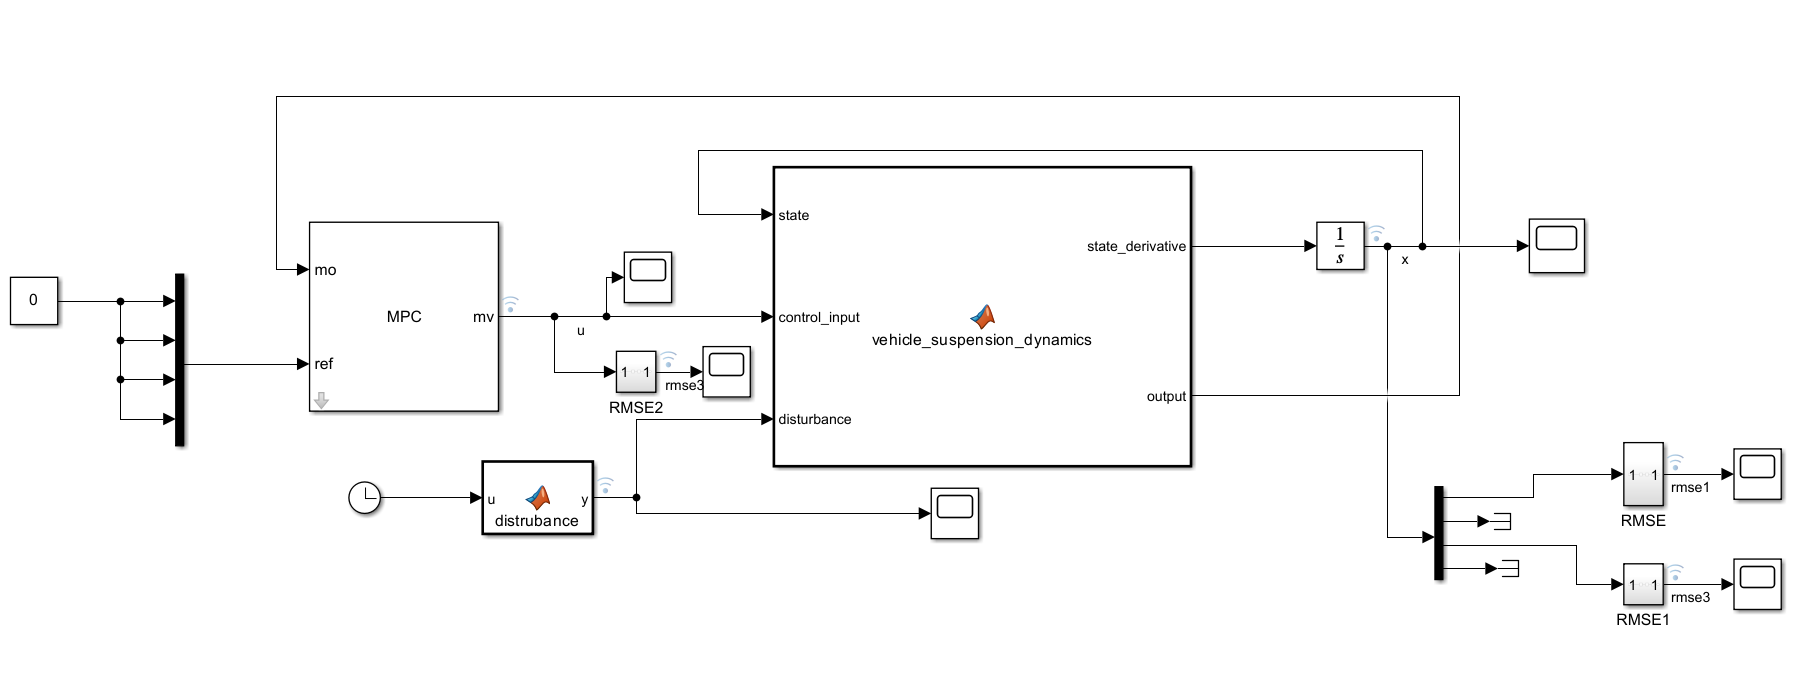
\includegraphics[width=1\linewidth]{../img/1}
	\caption{بلوک دیاگرام LMPC}
	\label{fig:1}
\end{figure}
لازم به ذکر است که با توجه به محدودیت های متلب برای ابعاد ورودی ها، خروجی ها و حالت های سیستم، چهار خروجی برای سیستم تعریف شده است، اما خروجی چهارم که نیازی نیست در نظر گرفته شود با مقدار 0 در نظر گرفته می شود.
معادلات سیستم را به صورت زیر در یک سیستم تعریف می کنیم.
\begin{figure}[H]
	\centering
	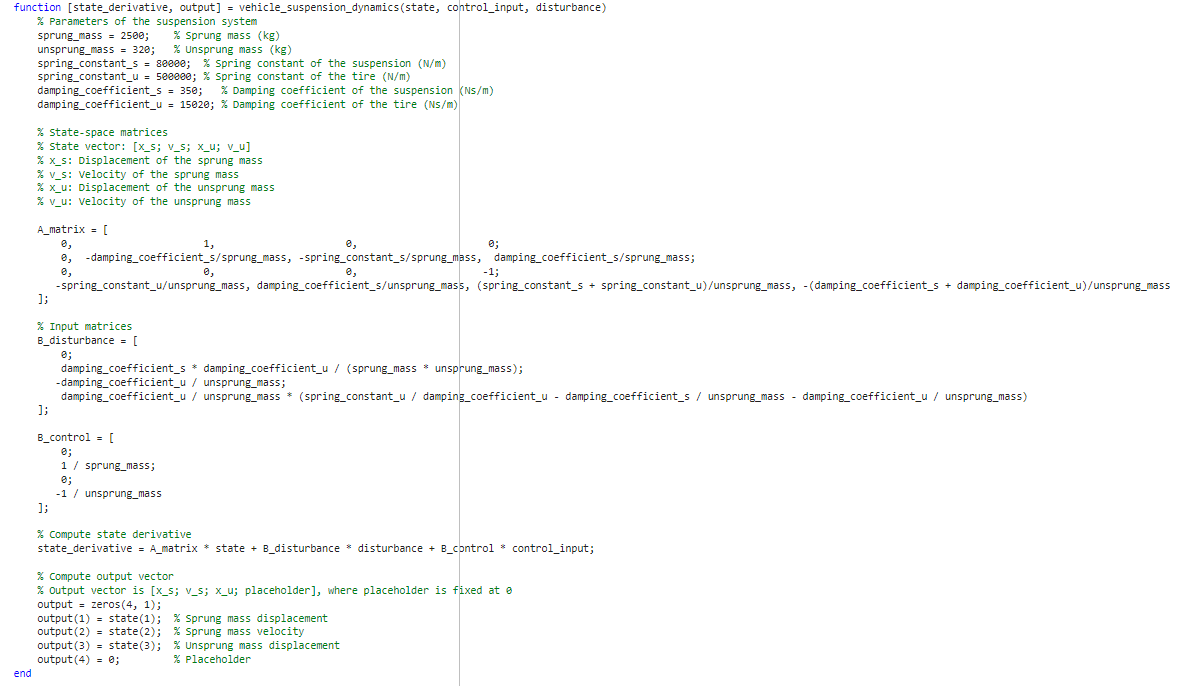
\includegraphics[width=1\linewidth]{../img/2}
	\caption{کد پلنت سیستم}
	\label{fig:2}
\end{figure}
همچنین، اغتشاش وارد شده به سیستم توسط کد زیر ایجاد می شود.

\begin{figure}[H]
	\centering
	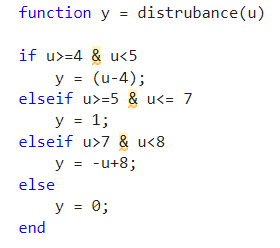
\includegraphics[width=0.4\linewidth]{../img/3}
	\caption{اغتشاش}
	\label{fig:3}
\end{figure}
در ادمه، با طراحی کنترلر MPC برای این سیستم با تنظیمات زیر، می توانیم نتایج به دست آمده از سیستم را مشاهده کنیم:

\begin{figure}[H]
	\centering
	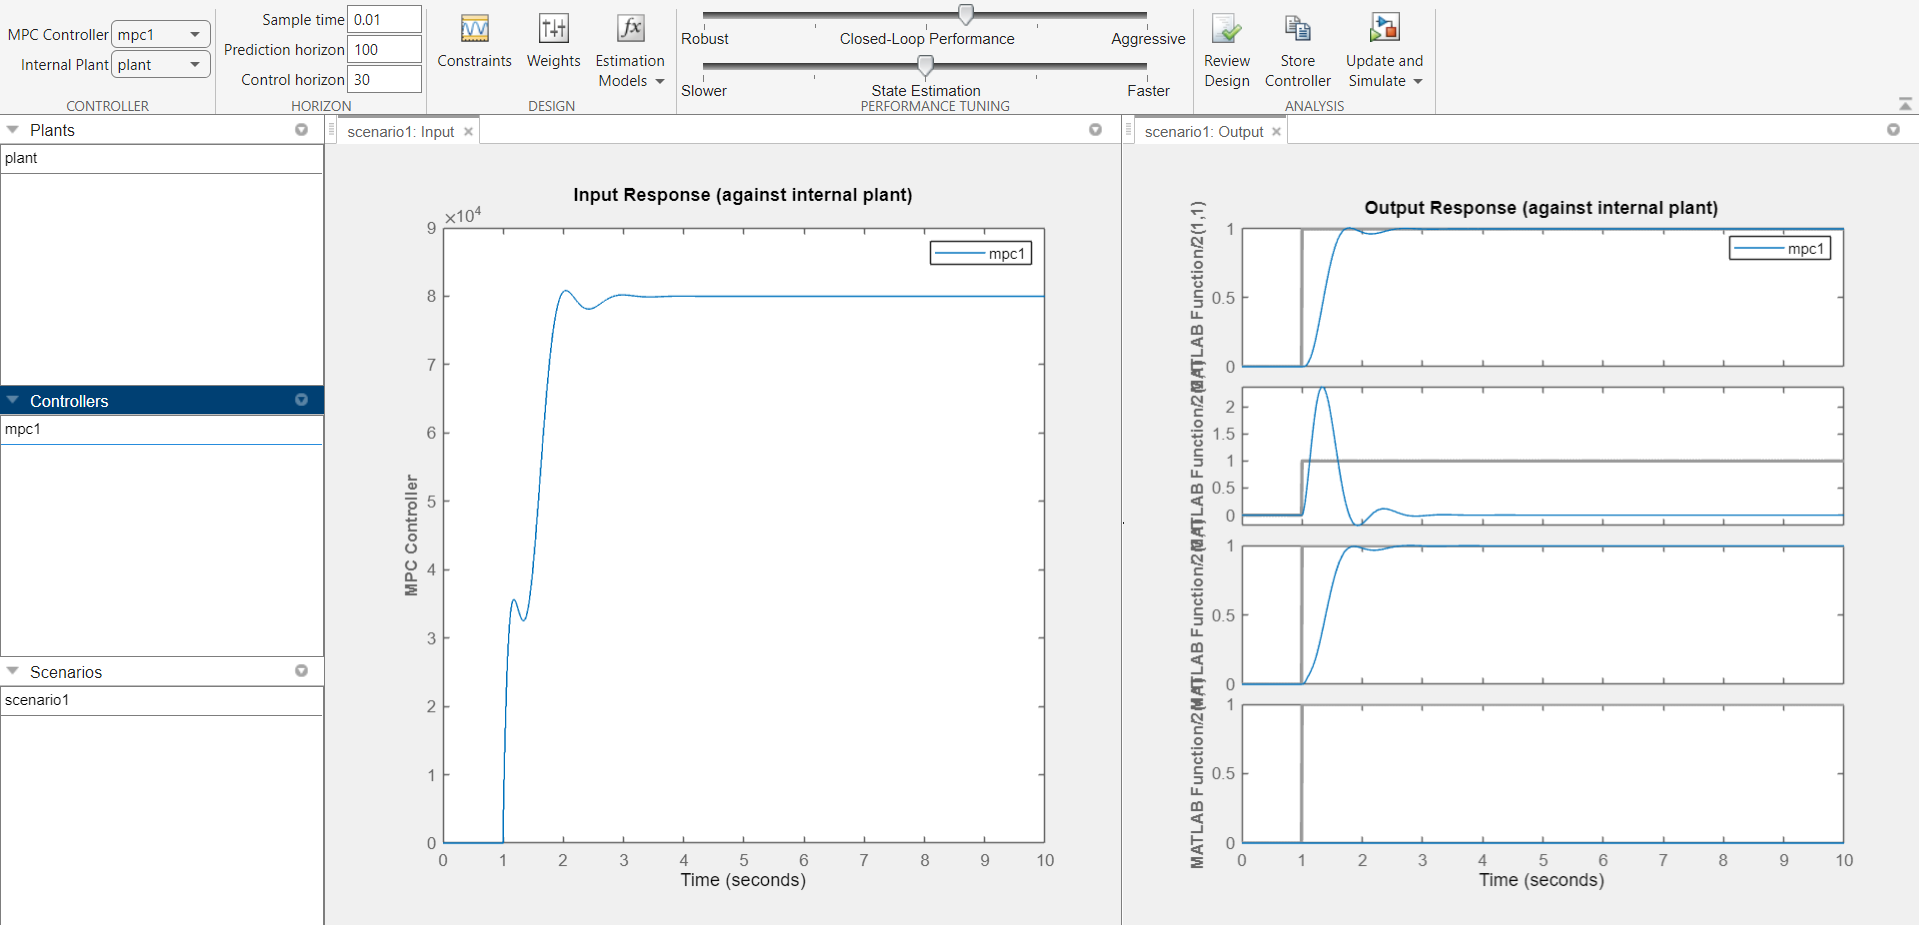
\includegraphics[width=1\linewidth]{../img/4}
	\caption{}
	\label{fig:4}
\end{figure}
همچنین باید توجه شود که قید هایی برای حالت اول سیستم در نظر گرفته شده است تا مقدار آن از 1 بیشتر نشود. 

\begin{figure}[H]
	\centering
	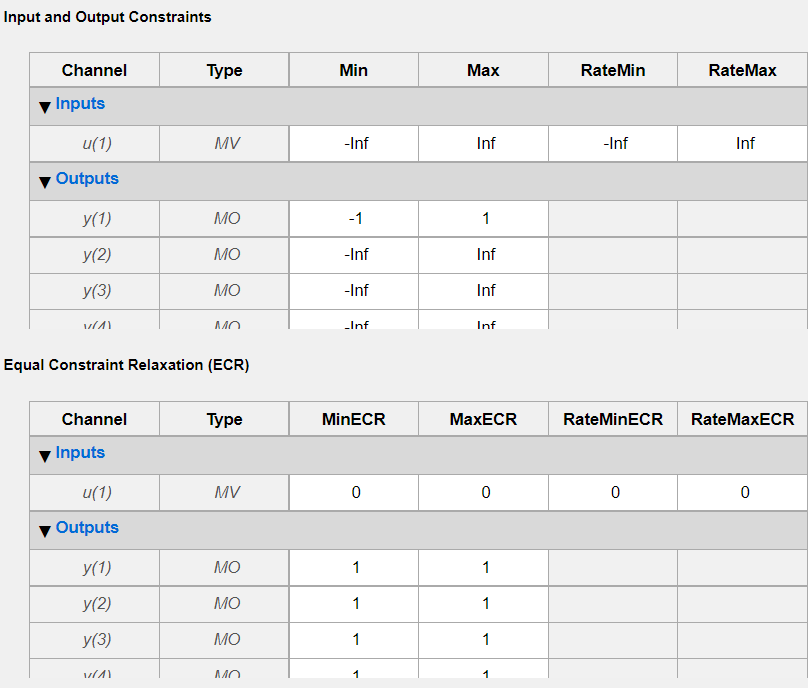
\includegraphics[width=1\linewidth]{../img/5}
	\caption{}
	\label{fig:5}
\end{figure}
با استفاده از سیستم تعریف شده، پاسخ های سیستم به صورت زیر به دست می آید.

\begin{figure}[H]
	\centering
	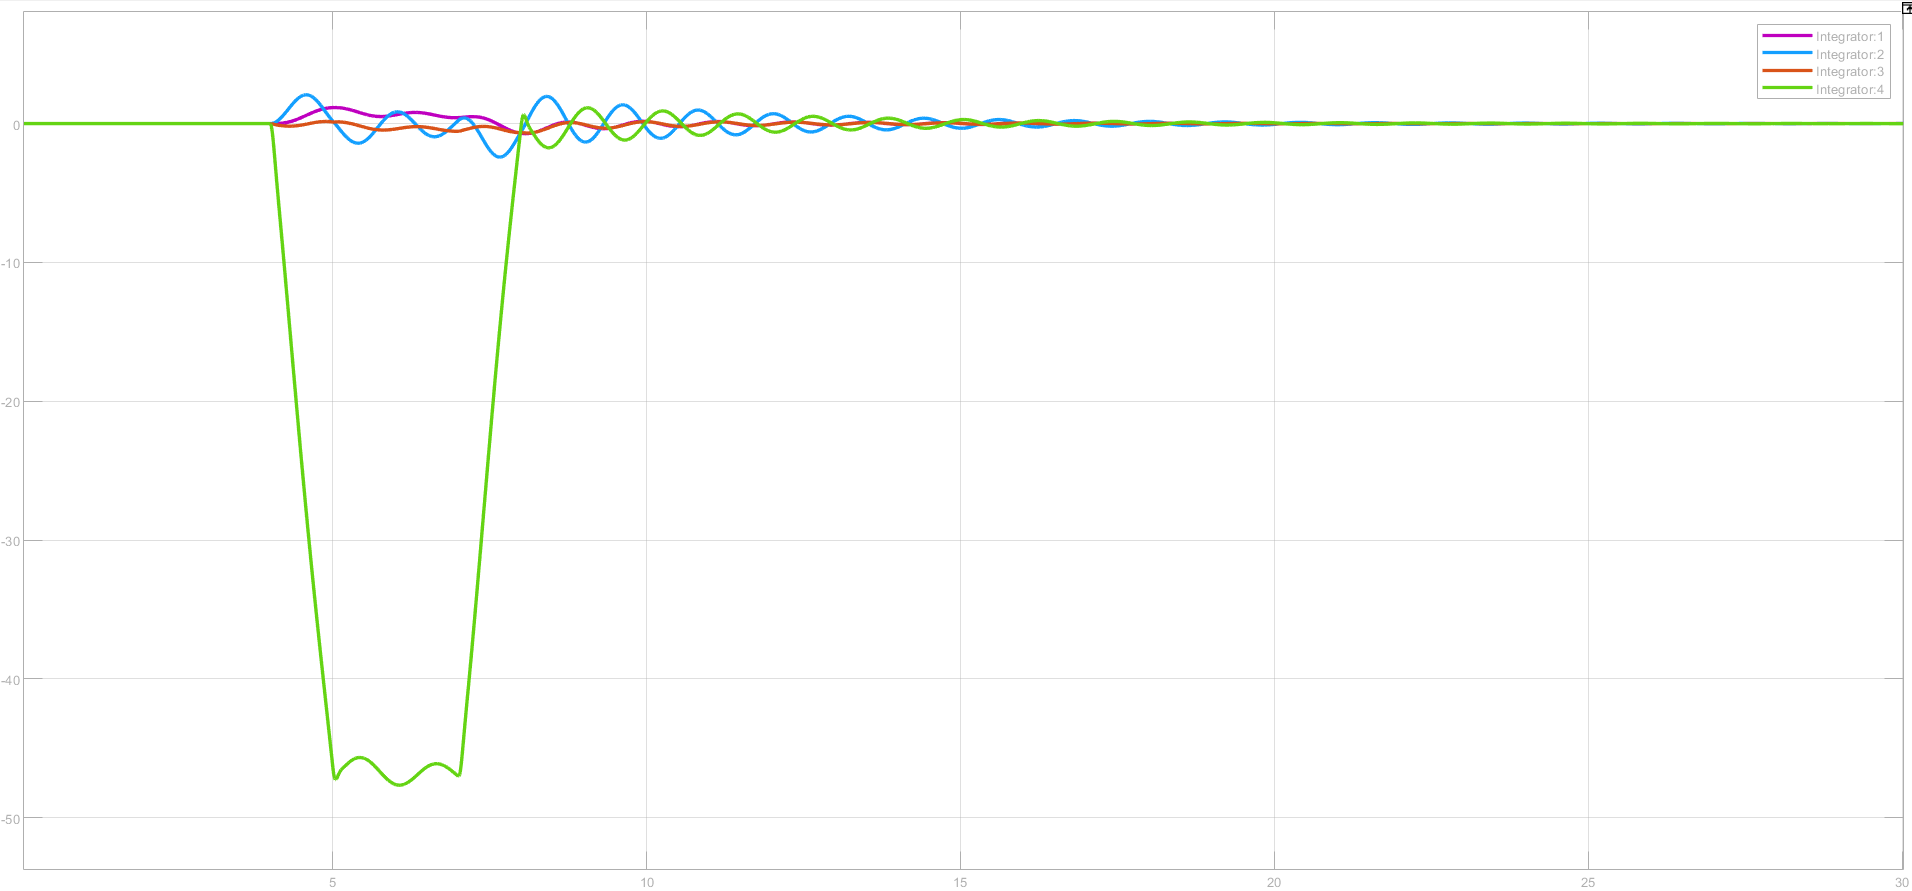
\includegraphics[width=1\linewidth]{../img/6}
	\caption{}
	\label{fig:6}
\end{figure}
همچنین نمودار تلاش کنترلی سیستم یه صورت زیر به دست می آید.

\begin{figure}[H]
	\centering
	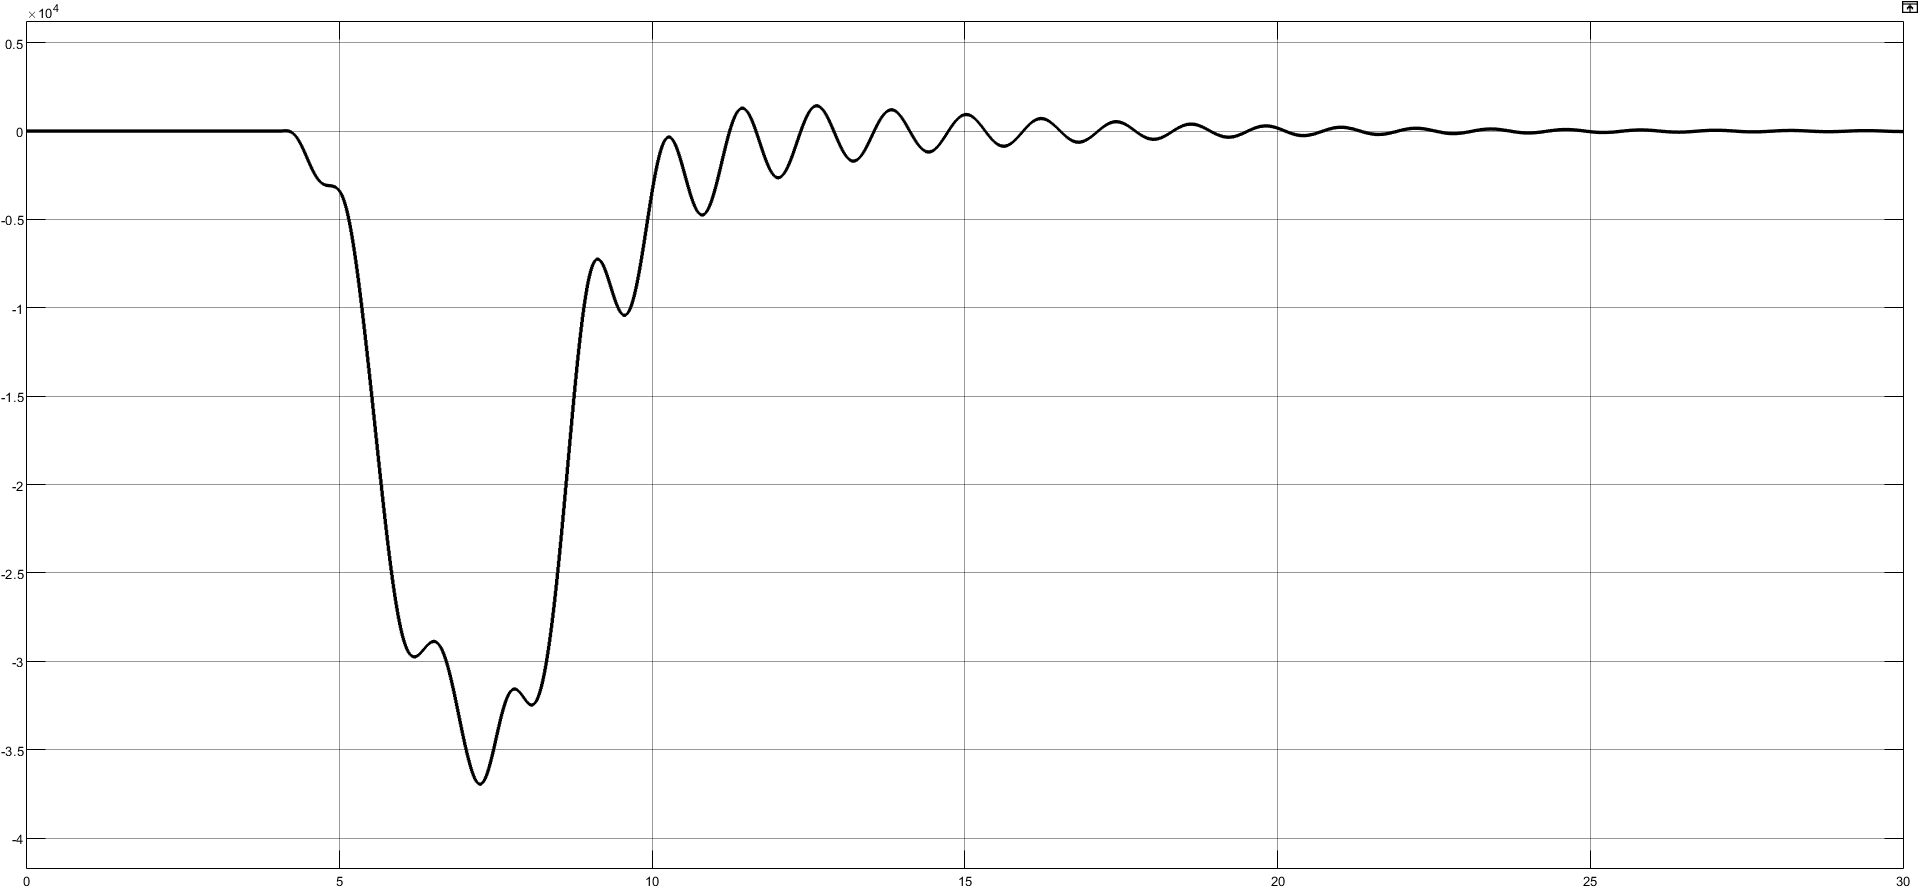
\includegraphics[width=1\linewidth]{../img/7}
	\caption{}
	\label{fig:7}
\end{figure}

با در اختیار داشتن نتایج به دست آمده و به منظور تحلیل این نتایج، کنترلر PID نیز برای سیستم طراحی و بررسی می شود. دیاگرام این سیستم به شرح زیر خواهد بود:

\begin{figure}[H]
	\centering
	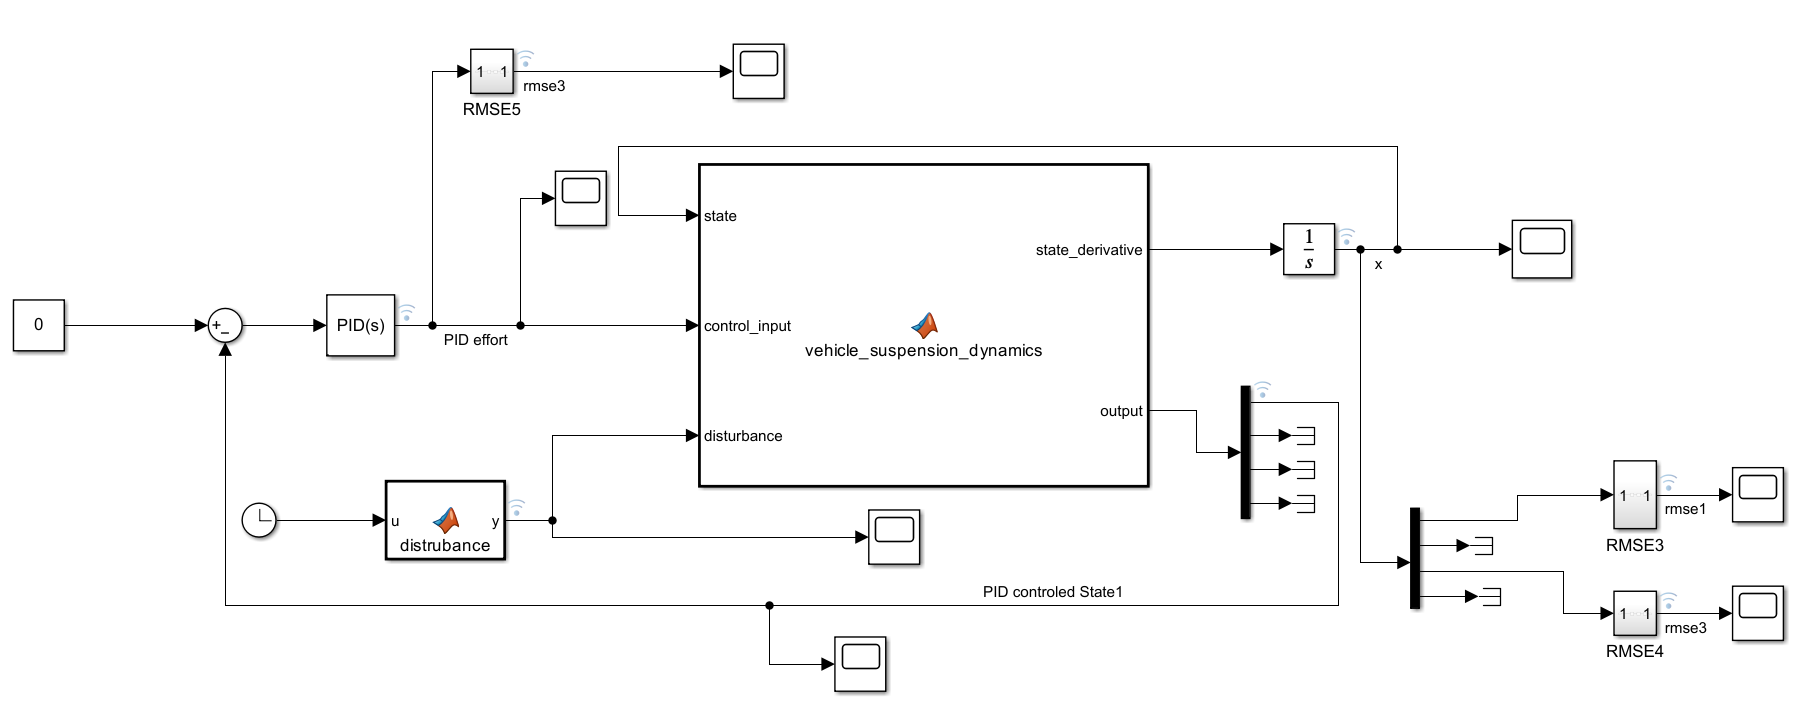
\includegraphics[width=1\linewidth]{../img/8}
	\caption{}
	\label{fig:8}
\end{figure}

لازم به ذکر است که برای این سیستم، تنها حالت اول به عنوان خروجی سیستم در نظر گرفته شده است. پاسخ سیستم به صورت زیر به دست می آید و مشاهده می شود که می تواند به خوبی اغتشاش وارد شده را رفع کند. اما با در نظر گرفتن ضرایب PID و همچنین نمودار تلاش کنترلی مشاهده می شود که در نهایت این کنترلر در سیستم های واقعی قابل پیاده سازی نمی باشد.

\begin{figure}[H]
	\centering
	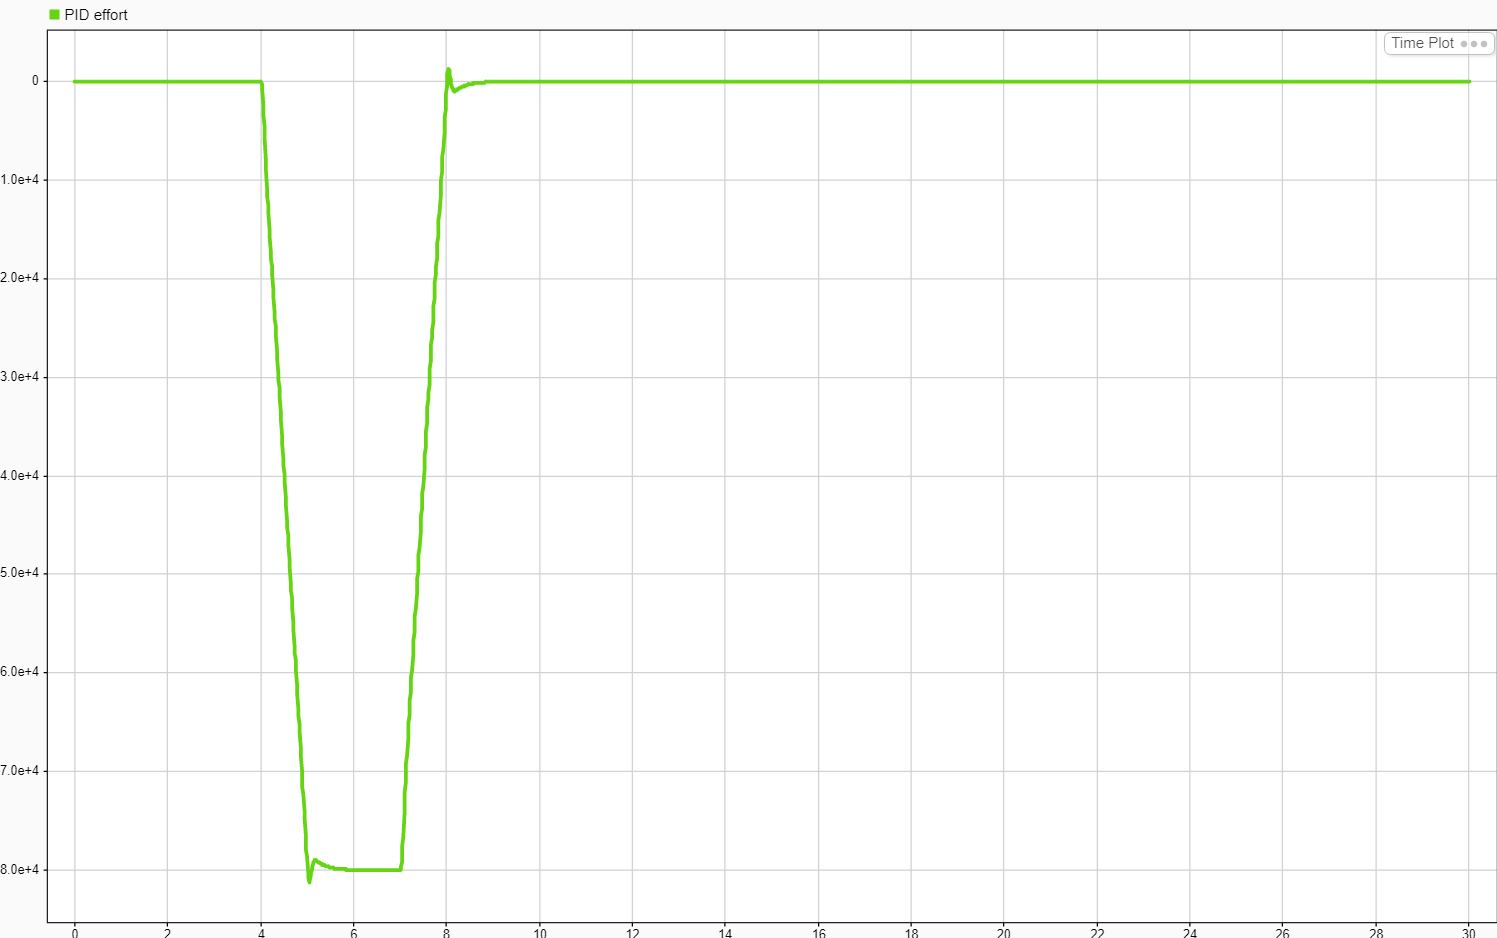
\includegraphics[width=1\linewidth]{../img/9}
	\caption{}
	\label{fig:9}
\end{figure}

\begin{figure}[H]
	\centering
	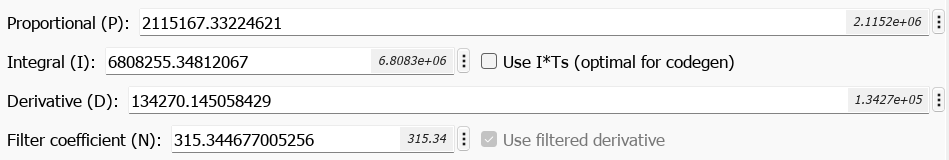
\includegraphics[width=0.7\linewidth]{../img/10}
	\caption{}
	\label{fig:10}
\end{figure}

\begin{figure}[H]
	\centering
	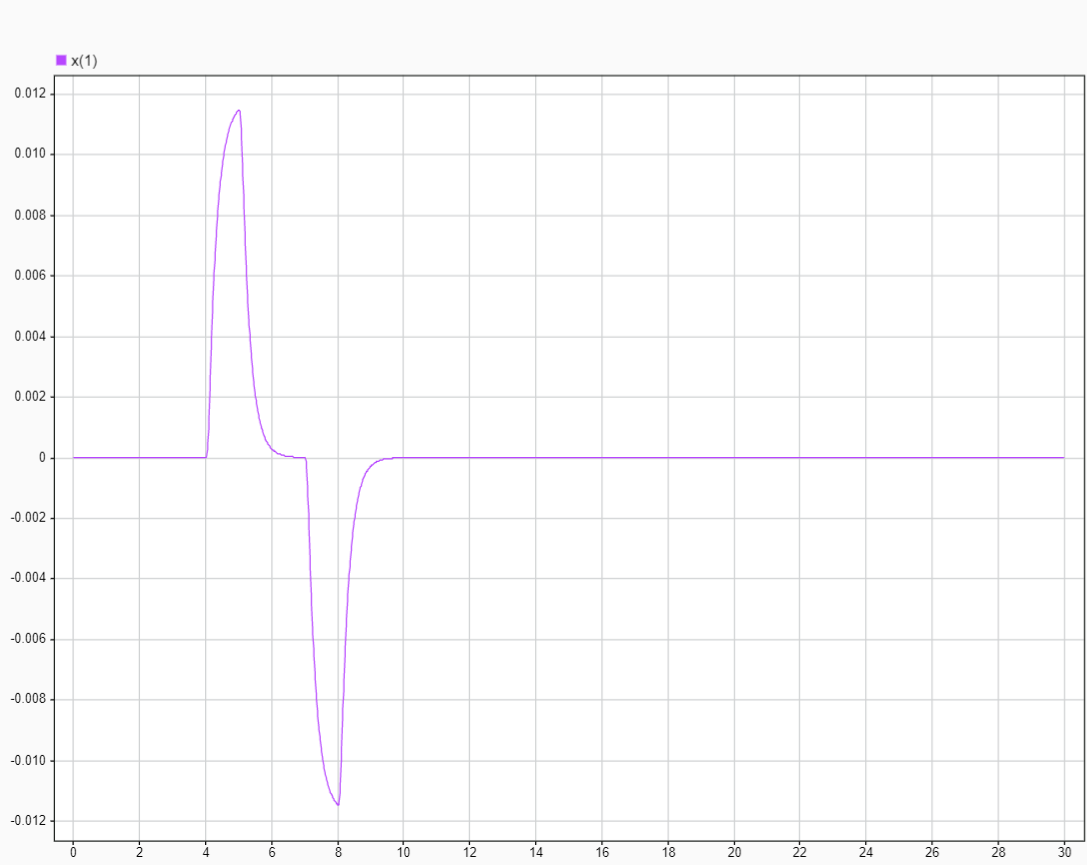
\includegraphics[width=1\linewidth]{../img/11}
	\caption{}
	\label{fig:11}
\end{figure}

در اینجا با در نظر گرفتن نتایج به دست آمده از MPC و PID می توانیم مقایسه ای در عملکرد آنها داشته باشیم.
نتایج به دست امده از خروجی کنترلی حالت اول با این دو کنترلر و تلاش کنترلی برای رفع آن به صورت زیر خواهد بود.

\begin{figure}[H]
	\centering
	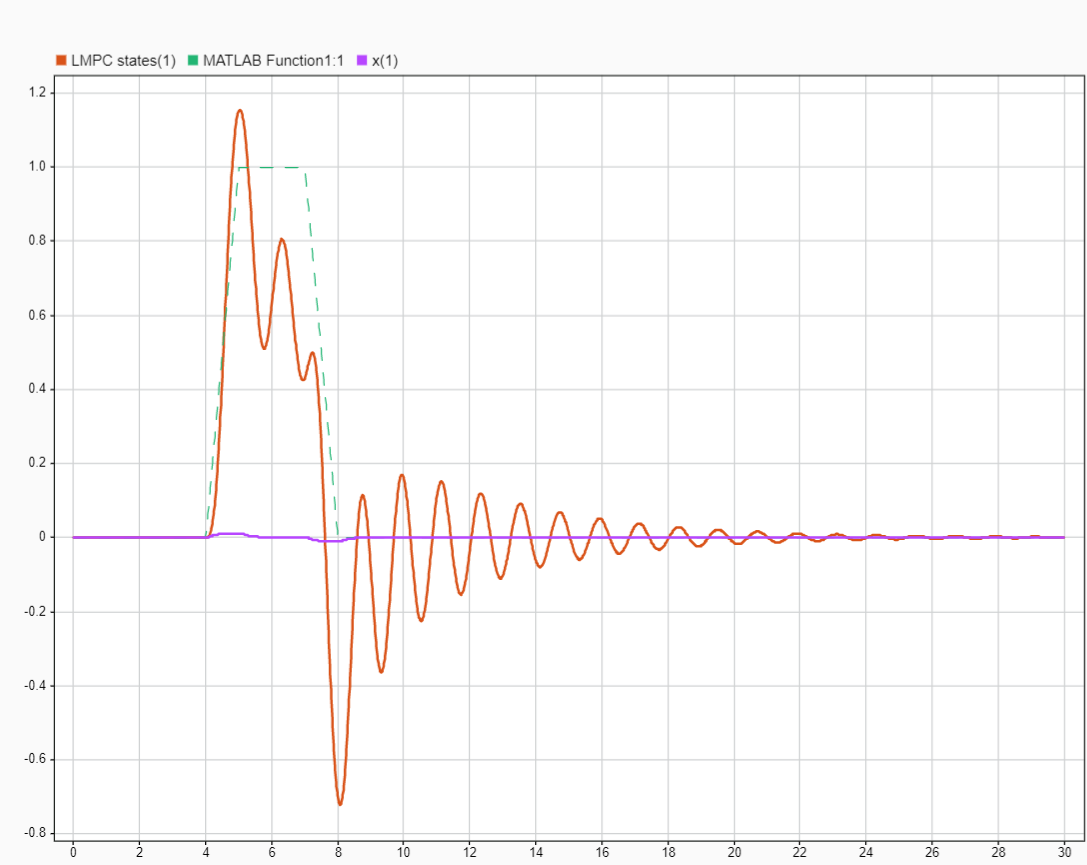
\includegraphics[width=1\linewidth]{../img/13}
	\caption{}
	\label{fig:13}
\end{figure}

\begin{figure}[H]
	\centering
	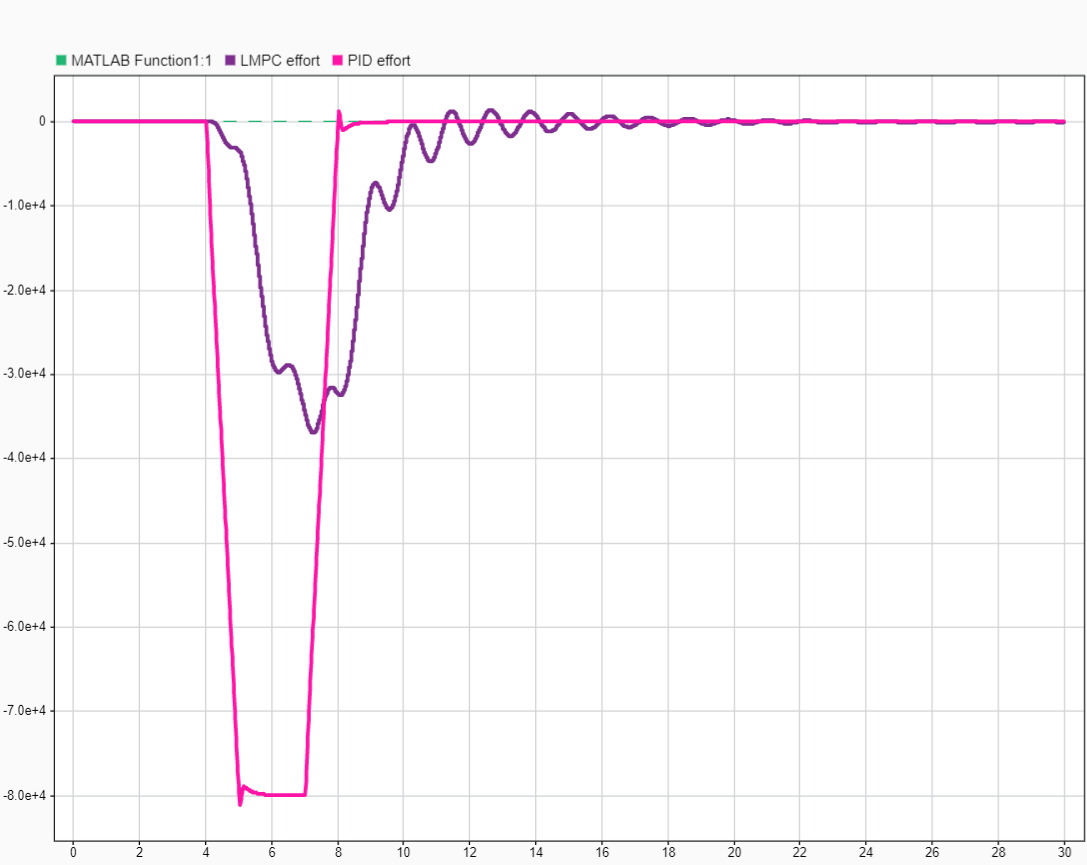
\includegraphics[width=1\linewidth]{../img/14}
	\caption{}
	\label{fig:14}
\end{figure}

همچنین مقادیر RMSE برای این دو کنترلر در دو حالت مورد نظر به صورت زیر به دست می آید.

\begin{figure}[H]
	\centering
	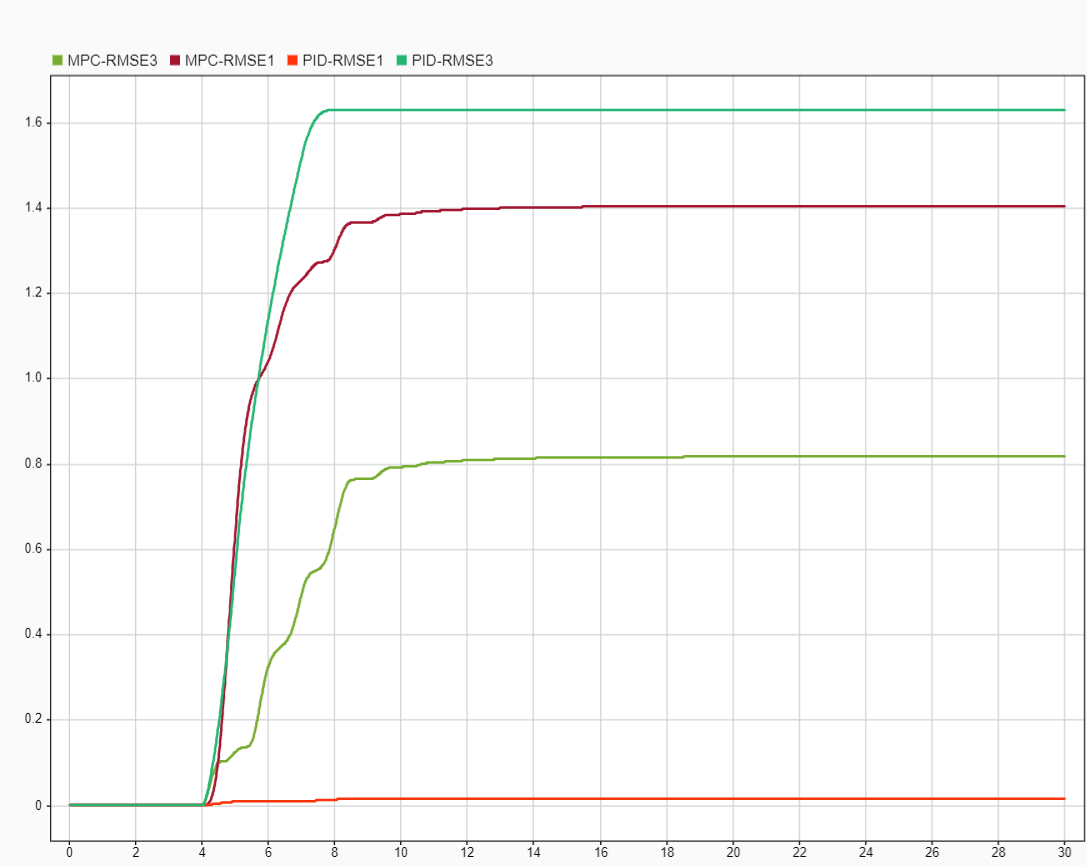
\includegraphics[width=1\linewidth]{../img/15}
	\caption{}
	\label{fig:15}
\end{figure}
نتایج به دست آمده نشان می ددهد که مقادیر RMSE برای کنترلر MPC بیشتر از کنترلر PID است. 
همچنین، مقدار RMSE برای ورودی کنترلرها به صورت زیر خواهد بود:

\begin{figure}[H]
	\centering
	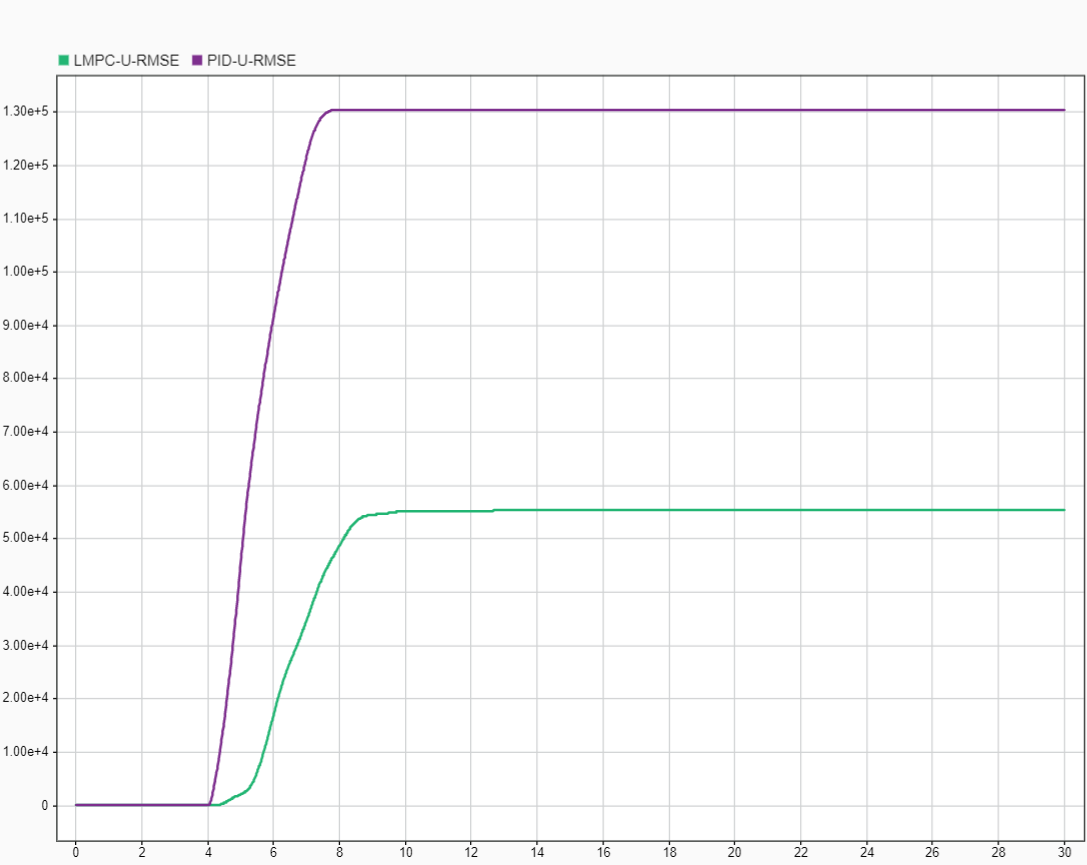
\includegraphics[width=1\linewidth]{../img/16}
	\caption{}
	\label{fig:16}
\end{figure}
در نتیجه دیاگرام های سیستم ها با تجه به تغییرات اعمال شده به صورت زیر برای دو کنترلر خواهد بود.

\begin{figure}[H]
	\centering
	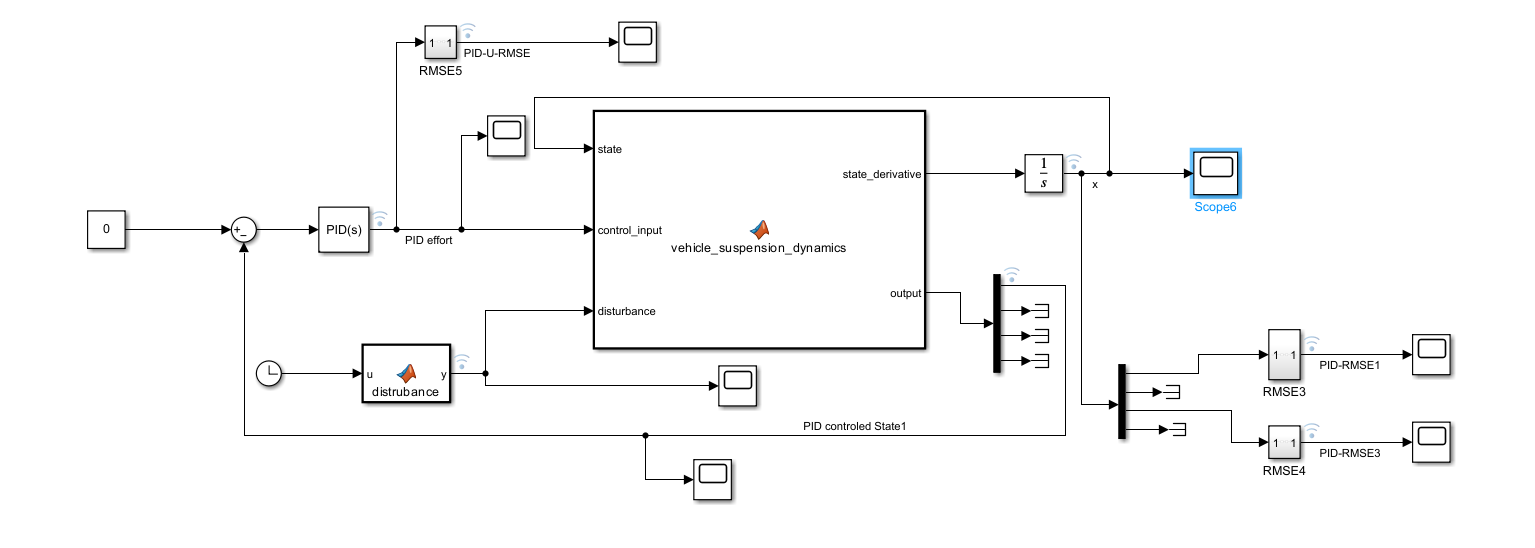
\includegraphics[width=1\linewidth]{../img/17}
	\caption{}
	\label{fig:17}
\end{figure}

\begin{figure}[H]
	\centering
	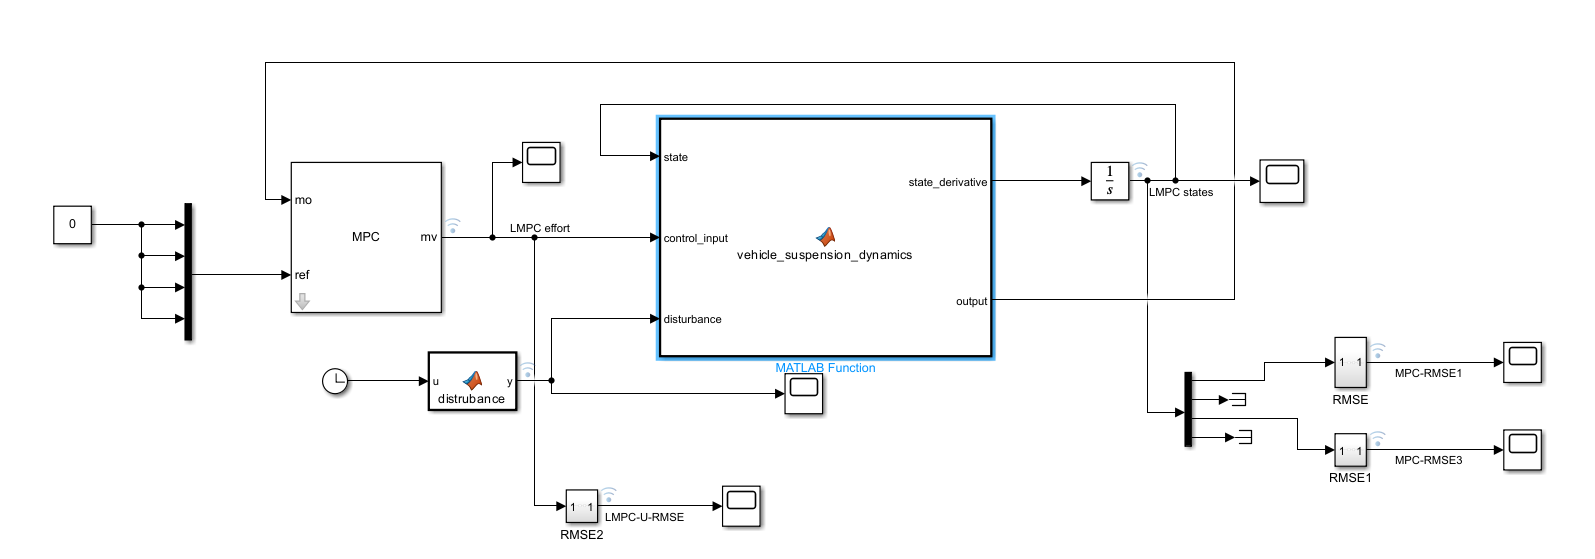
\includegraphics[width=1\linewidth]{../img/18}
	\caption{}
	\label{fig:18}
\end{figure}

\subsection*{سوال دوم}
در این بخش، با افزودن یک کنترلر PID به MPC و تشکیل یک کنترلر $Tube MPC$، مجددا نتایج را بررسی می کنیم. بنابراین، ساختار سیستم طراحی شده به صورت زیر خواهد بود:

\begin{figure}
	\centering
	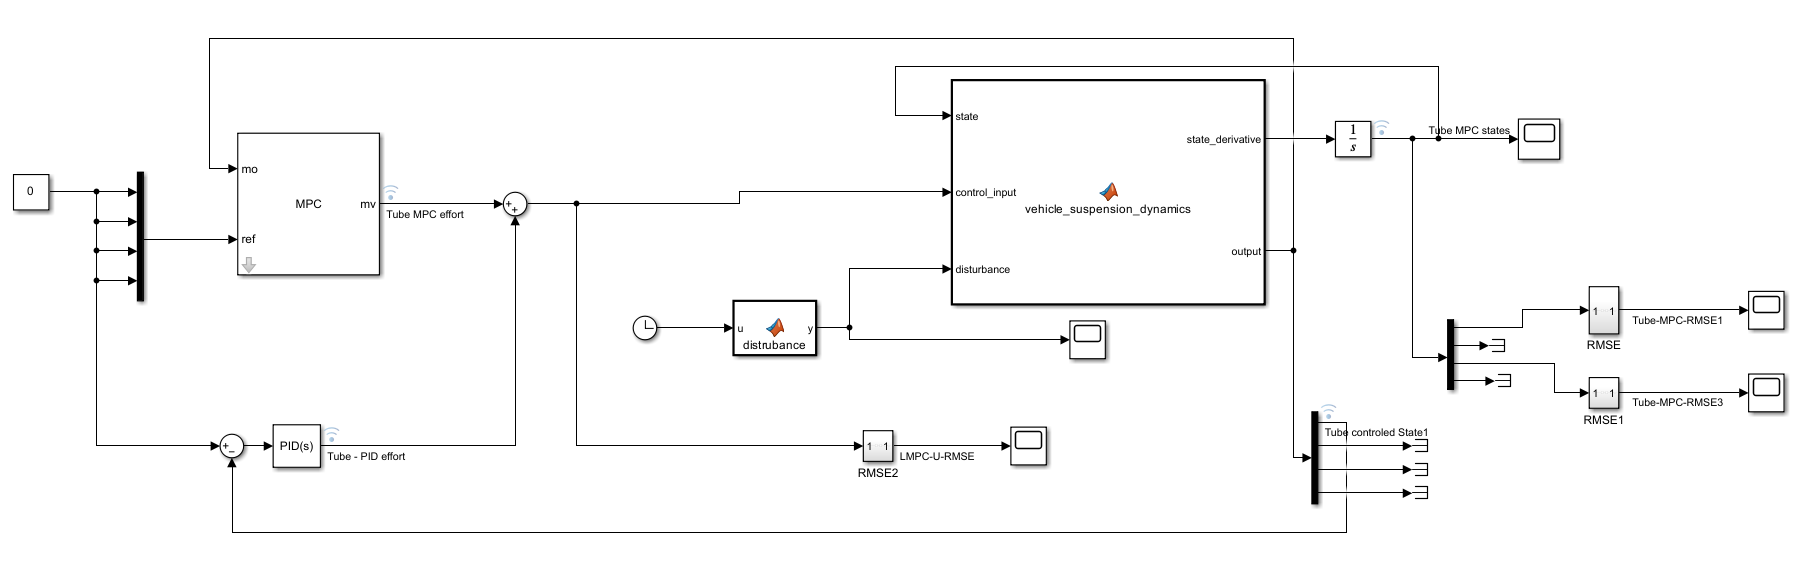
\includegraphics[width=1\linewidth]{../img/19}
	\caption{}
	\label{fig:19}
\end{figure}
در ادامه، با تنظیم مجدد کنترلر MPC و PID، کنترلر ها را مجددا طراحی می کنیم. تنظیم های کنترلر PID به صورت زیر خواهد بود.
\begin{figure}
	\centering
	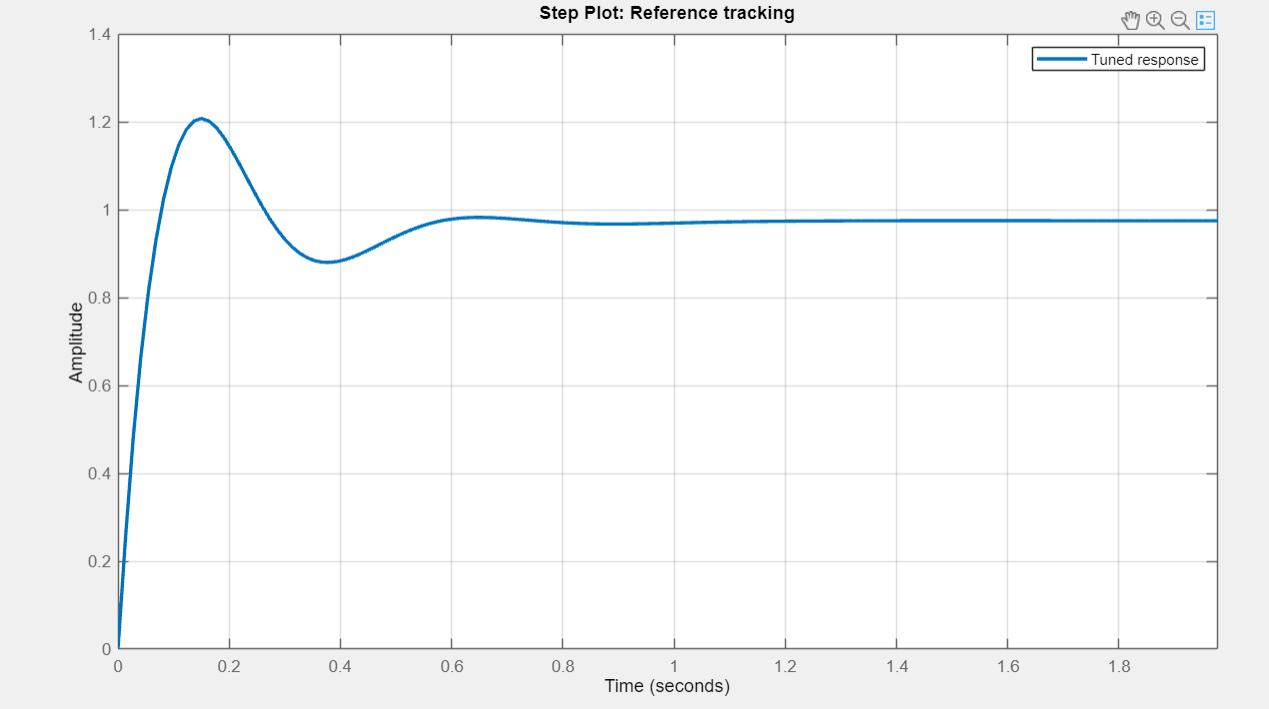
\includegraphics[width=1\linewidth]{../img/20}
	\caption{}
	\label{fig:20}
\end{figure}

\begin{figure}
	\centering
	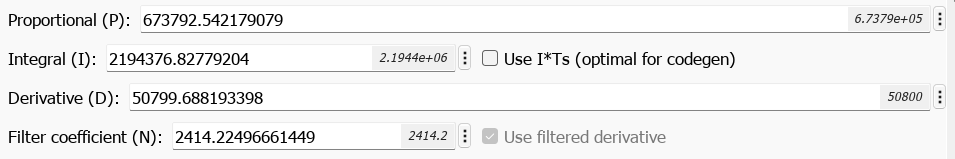
\includegraphics[width=1\linewidth]{../img/21}
	\caption{}
	\label{fig:21}
\end{figure}
تنظیمات MPC به صورت زیر خواهد بود:

\begin{figure}
	\centering
	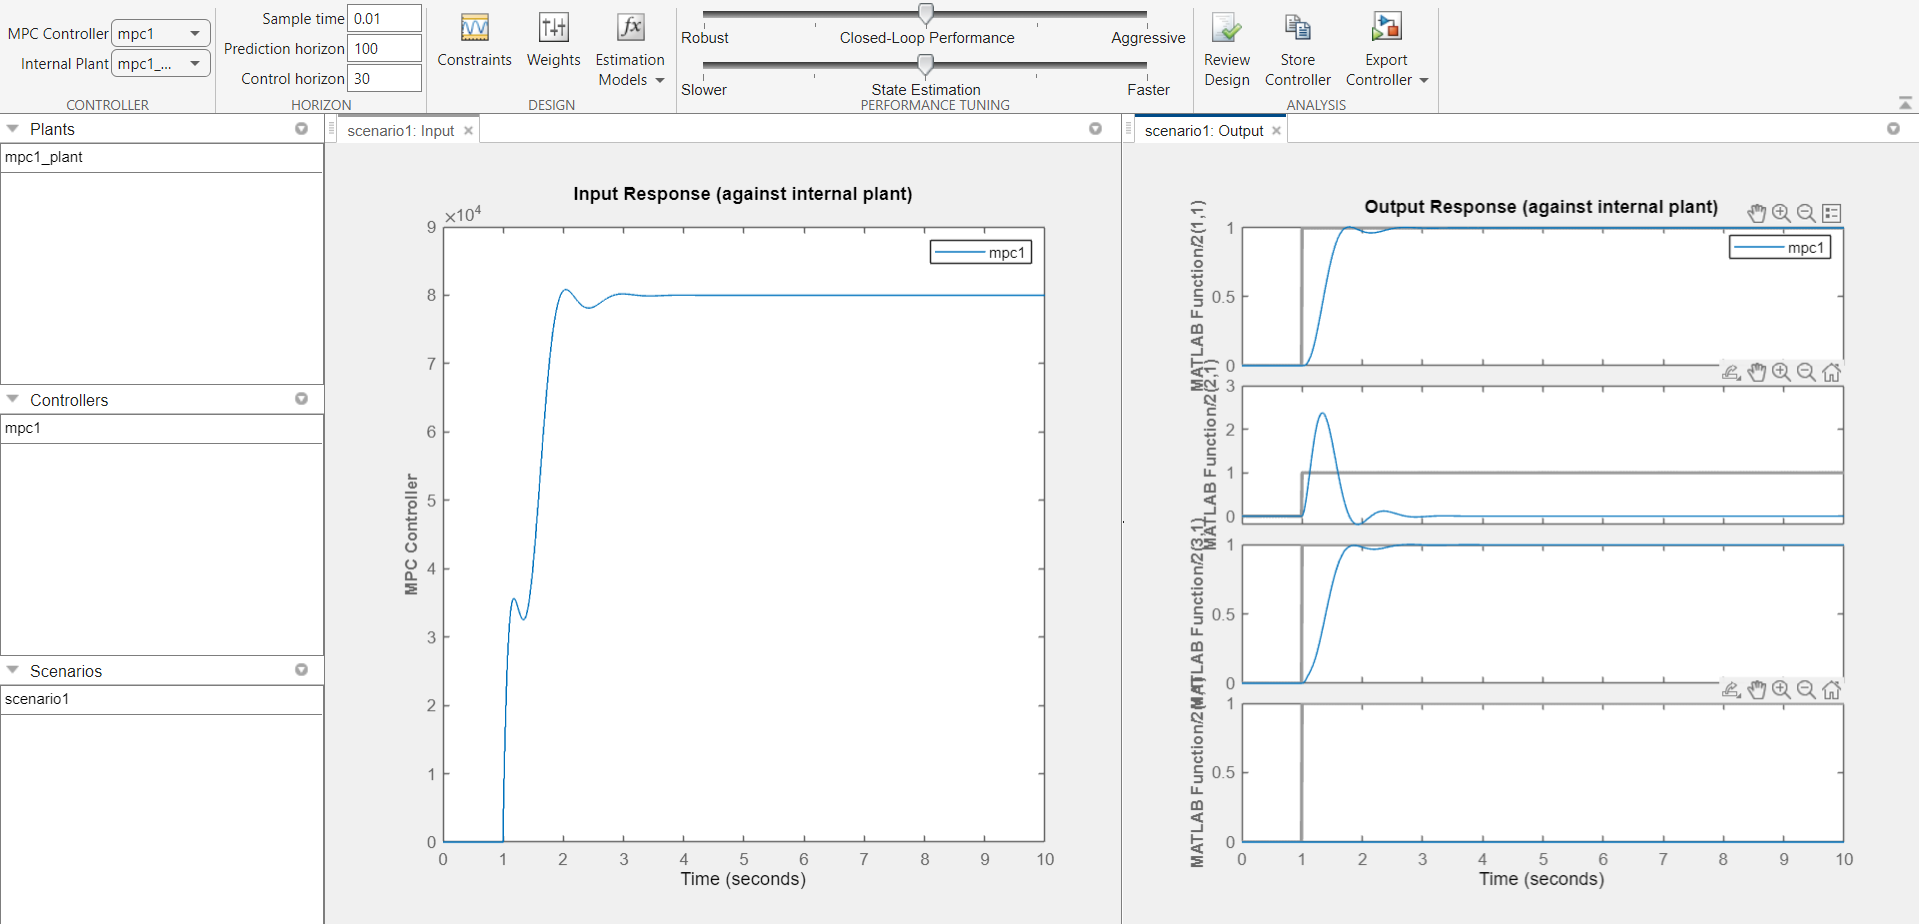
\includegraphics[width=1\linewidth]{../img/22}
	\caption{}
	\label{fig:22}
\end{figure}
% TODO: \usepackage{graphicx} required
\begin{figure}
	\centering
	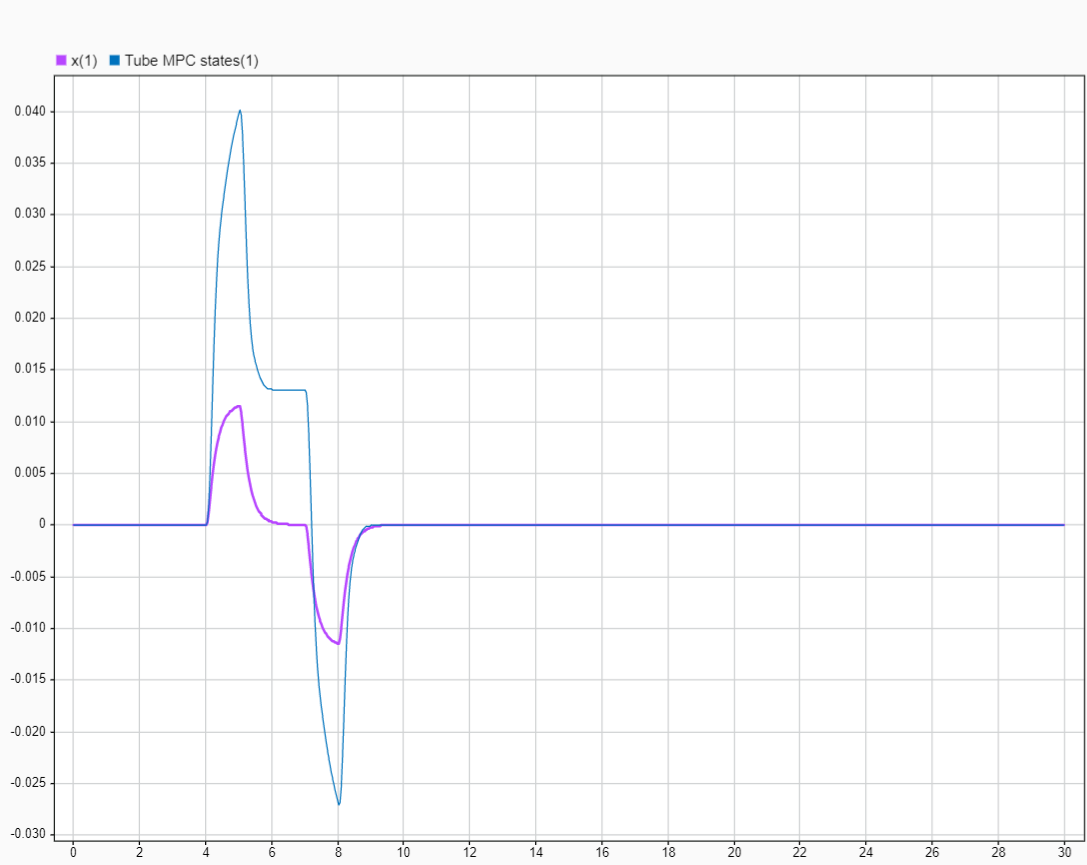
\includegraphics[width=1\linewidth]{../img/23}
	\caption{}
	\label{fig:23}
\end{figure}
% TODO: \usepackage{graphicx} required
\begin{figure}
	\centering
	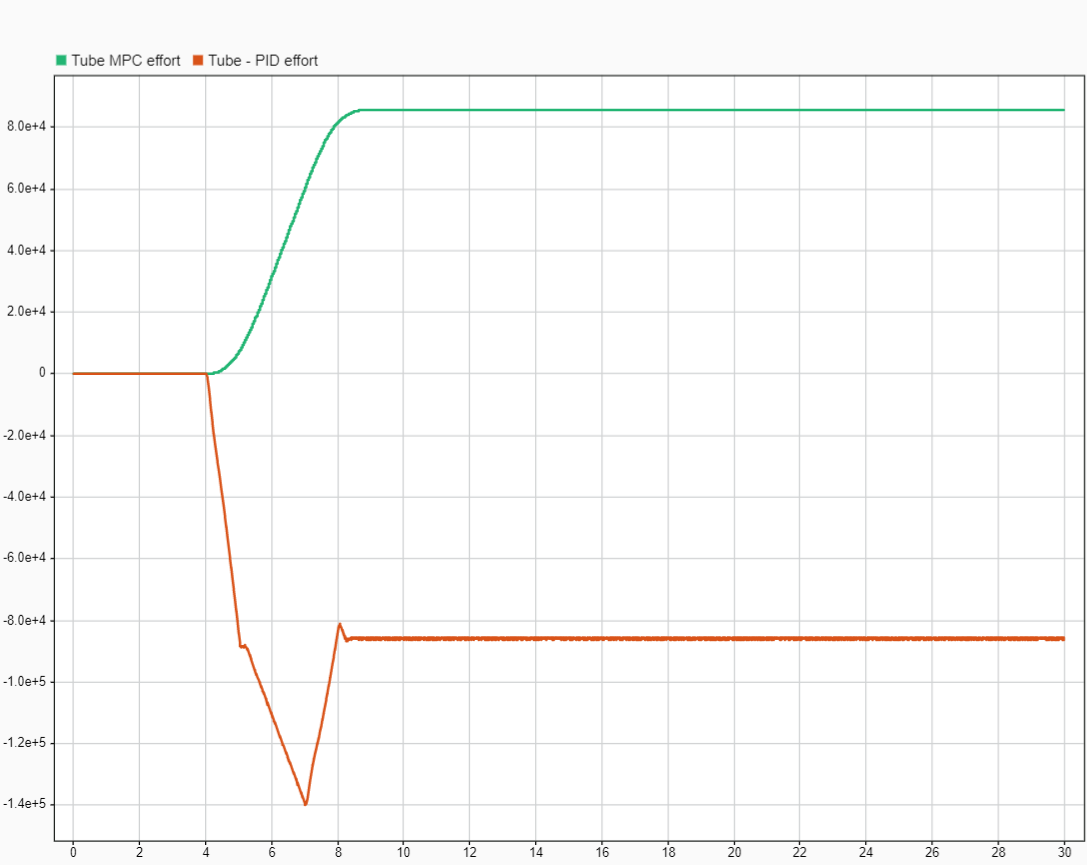
\includegraphics[width=1\linewidth]{../img/24}
	\caption{}
	\label{fig:24}
\end{figure}
% TODO: \usepackage{graphicx} required
\begin{figure}
	\centering
	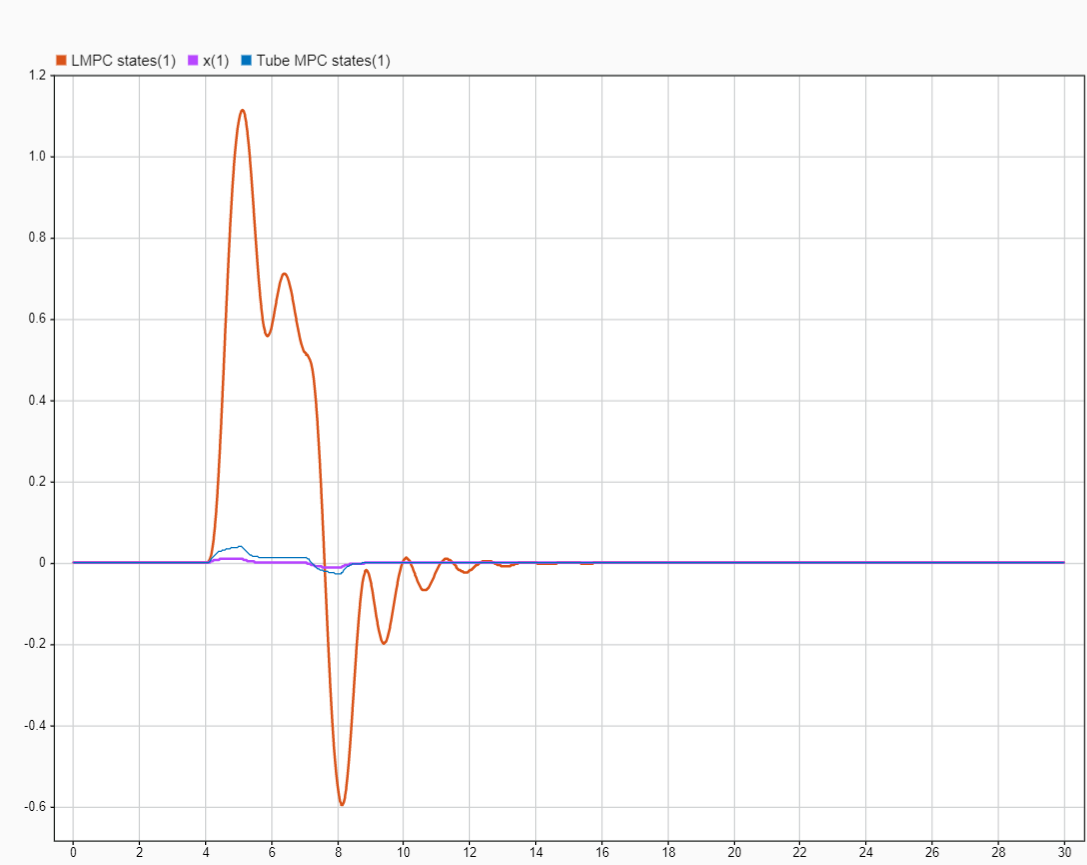
\includegraphics[width=1\linewidth]{../img/25}
	\caption{}
	\label{fig:25}
\end{figure}



















